\chapter{Progettazione}

\section{Diagramma delle classi}

\subsection{Package \texttt{incud.immutable}}
Gli oggetti delle classi che seguono rappresentano un insieme di dati che non cambiano, che non hanno uno stato quindi immutabili. Al posto di riempire le classi di metodi \texttt{get*}, sono stati resi pubblici gli attributi che non potranno essere comunque modificati dall'utilizzatore. Le collezioni vengono create coi metodi \texttt{Collections.unmodifiable*}.

Per quanto riguarda la classe \texttt{Disco}, il campo \texttt{autore} è una stringa che deve riferirsi ad un artista presente nel sistema. Alla creazione del disco viene difatti svolto un controllo di coerenza dei dati.

Per quanto riguarda la classe \texttt{Autore}, il campo \texttt{strumentiSuonati} di un autore \emph{non deve necessariamente rispecchiare} gli strumenti che suona nelle istanze di \texttt{Partecipazione}: può darsi che in una partecipazione di un dato autore ci sia uno strumento non presente nei suoi \texttt{strumentiSuonati}.

\begin{center}
    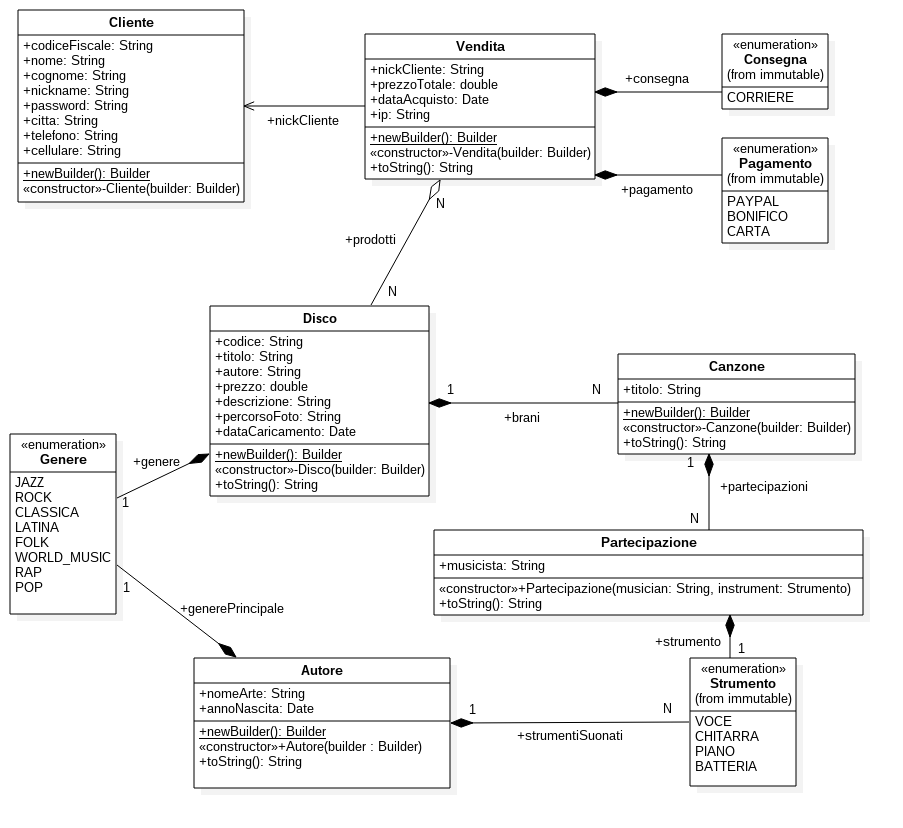
\includegraphics[width=0.9\textwidth]{diagram/classi-immutable.png}
\end{center}

\subsection{Package \texttt{incud.stato}}

Le classi del package (tutte signleton) tengono traccia dello stato del negozio: i dischi presenti nel negozio, le scorte, i clienti registrati e le vendite effettuate.

\begin{center}
    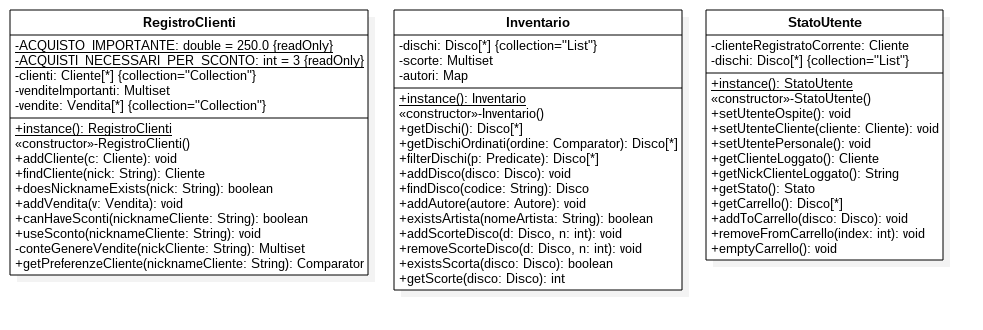
\includegraphics[width=\textwidth]{diagram/classi-stato.png}
\end{center}

\subsection{Package \texttt{incud.util} e \texttt{incud.io}}

Il package \texttt{incud.util} contiene metodi d'utilità, \texttt{incud.io} permette di caricare file e immagini dal filesystem, da internet e dall'interno del package. La classe \texttt{JsonLoader} fornisce il metodo \texttt{load} per caricare il database con dati di prova all'interno del sistema.

\begin{center}
    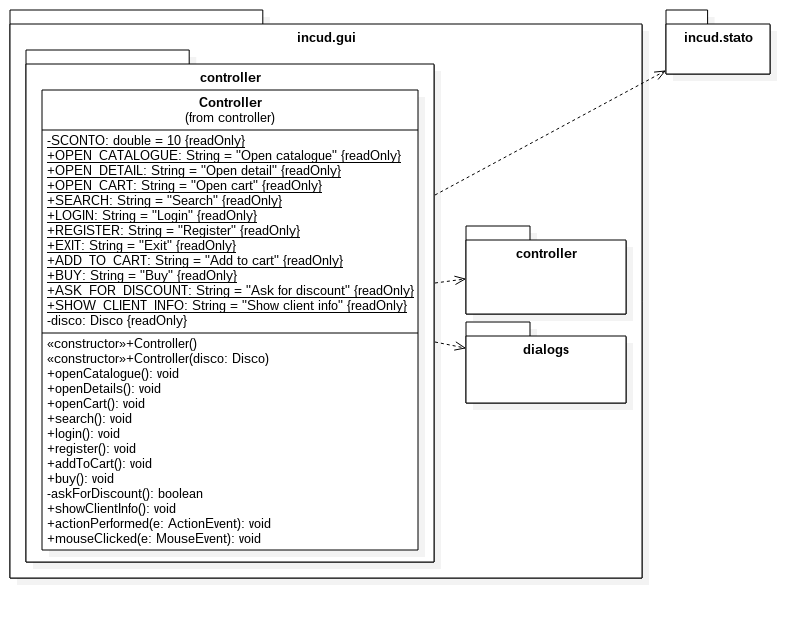
\includegraphics[width=\textwidth]{diagram/classi-util-io.png}
\end{center}

\subsection{Package \texttt{incud.gui}}

Il package \texttt{incud.gui} è organizzato come segue:
\begin{itemize}
    \item \texttt{incud.gui.controller} contiene la classe \texttt{Controller} che è l'unico \texttt{Action Listener} di tutte le classi del package. La classe utilizzatrice dovrà chiamare \texttt{setActionCommand(comm : String)} con parametro una delle costanti della classe \texttt{Controller}, a seconda di quale operazione deve essere compiuta.
    \item \texttt{incud.gui.dialog} contiene i dialog (classi che implementano \texttt{JDialog}) che chiedono agli utilizzatori di inserire dati. Tutti i dialog sono bloccanti \footnote{\texttt{http://docs.oracle.com/javase/tutorial/uiswing/misc/modality.html}}.
    \item \texttt{incud.gui.frame} contiene la classe \texttt{Frame} che è il \texttt{JFrame} (finestra) principale dell'applicazione e i pannelli usati al suo interno. La classe \texttt{Frame} implementa un layout manager \texttt{CardLayout} che permette di interscambiare i diversi pannelli (per il catalogo, per il carrello, ...).
\end{itemize}

\begin{center}
    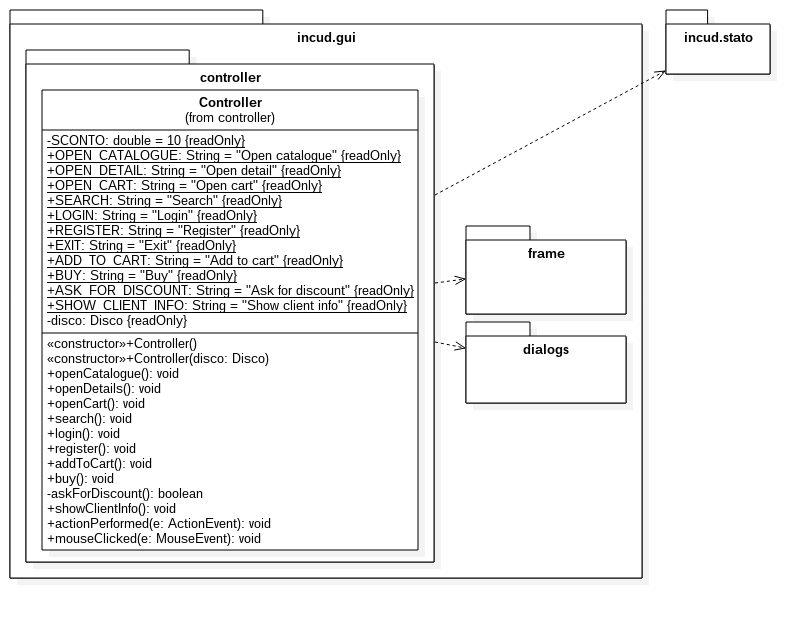
\includegraphics[width=\textwidth]{diagram/classi-gui.png}
\end{center}

\section{Pattern architetturali}

L'unico pattern architetturale utilizzato è MVC, che è anche intrinseco in Swing (la libreria grafica utilizzata). La classe \texttt{Frame} implementa la vista, l'ascoltatore \texttt{Controller} implementa il controller e il modello è dato dalle classi singleton all'interno di \texttt{incud.stato}.

\section{Pattern di progettazione}

\subsection{Pattern creazionali}

Nel package \texttt{incud.immutable} molte delle classi implementano il pattern Builder (senza parte Director, come per la classe \texttt{StringBuilder} di Java \footnote{https://stackoverflow.com/questions/4313172/builder-design-pattern-why-do-we-need-a-director}). I metodi ritornano l'istanza del builder stesso per avere un'interfaccia \emph{Fluent} \footnote{\texttt{https://en.wikipedia.org/wiki/Fluent\_interface}}.

Nel package \texttt{incud.stato} tutte le classi implementano il pattern Singleton.

\subsection{Pattern strutturali}

La classe \texttt{DataLoader} implementa il pattern Façade per facilitare l'apertura del database e il recupero del suo contenuto.

\subsection{Pattern comportamentali}

L'interfaccia \texttt{incud.util.Filter} e le sue implementazioni implementano il pattern Strategy. La classe \texttt{Sieve} implementa il pattern Template in modo simile a quanto fa il metodo \texttt{Collections.sort}.

\section{Dettagli delle principali operazioni}

\begin{center}
    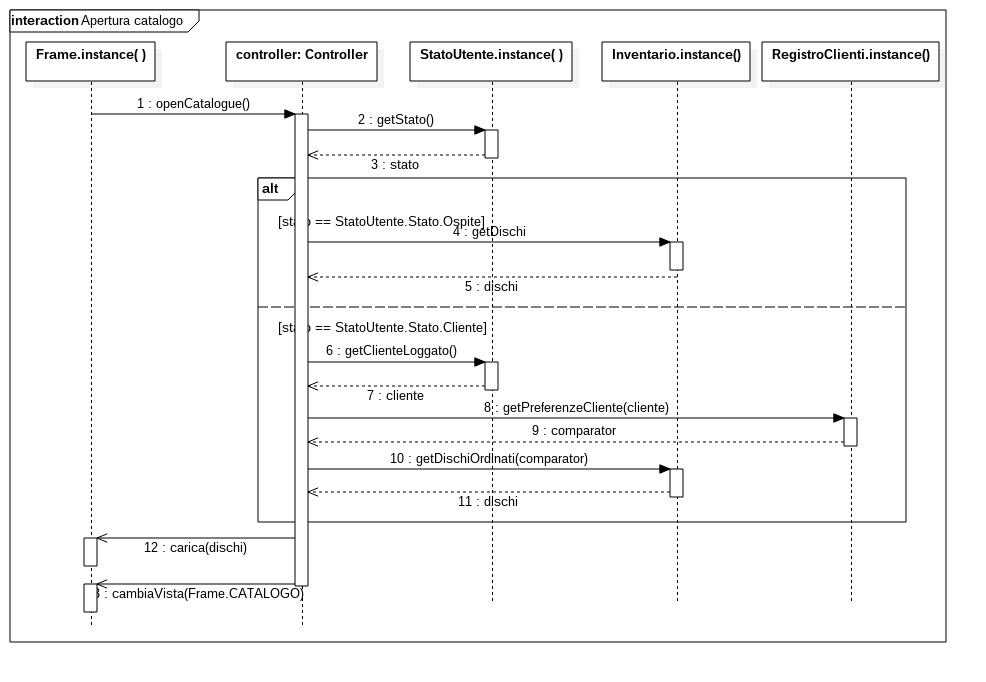
\includegraphics[width=\textwidth]{diagram/seq-apertura-catalogo.png}
\end{center}

\begin{center}
    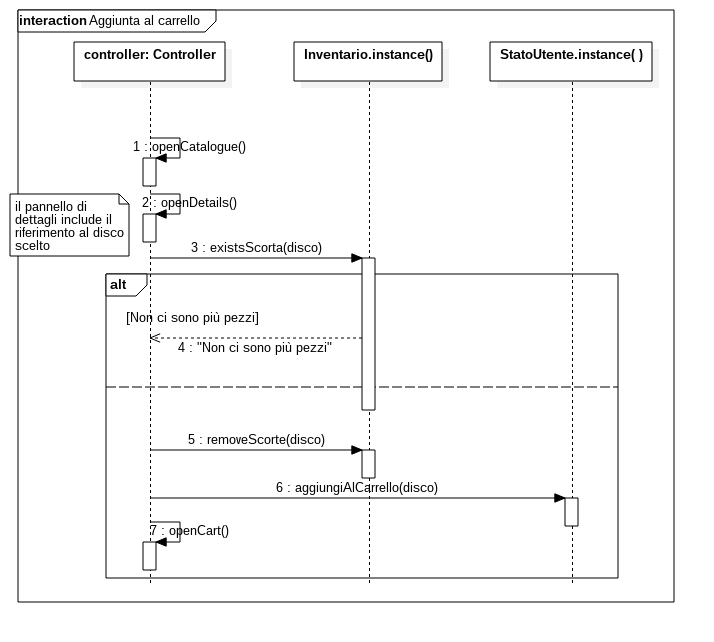
\includegraphics[width=0.98\textwidth]{diagram/seq-aggiunta-carrello.png}
\end{center}

\begin{center}
    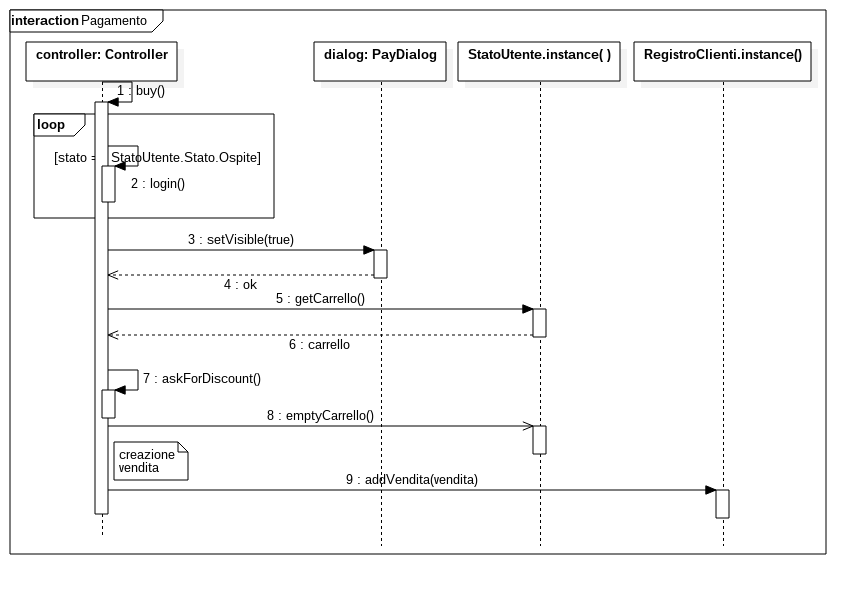
\includegraphics[width=\textwidth]{diagram/seq-pagamento.png}
\end{center}


